\section{Mathematical model and numerical experiments}
\label{model}

In this discourse, we focus our attention on a single chondrocyte cell
residing in deep regions of cartilage. This cartilage environment is
modelled simply by (fixed) external concentrations \Nao, \Ko, \Cao,
and \Ho. Values for these concentrations are chosen within
physiologically-relevant ranges (Hall et. al.). We are interested in
studying the behaviour of cell under this environment, in particular
looking at how the flux of these ions through membrane channels
changes their internal concentrations over time and how this changes
the cell's membrane potential.

\begin{figure}
  \centering
  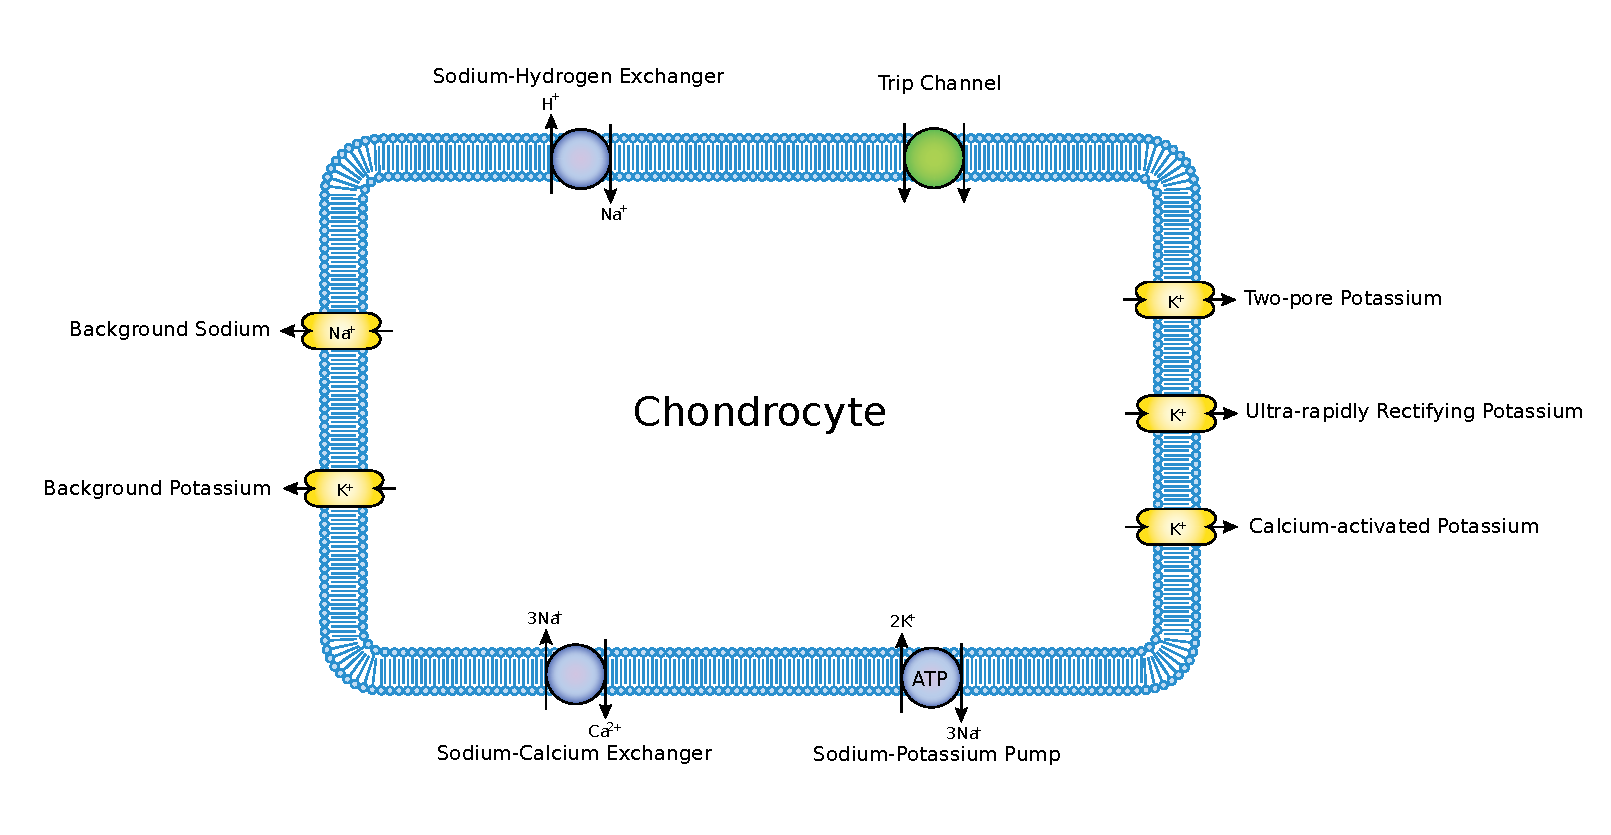
\includegraphics[width=\textwidth]{../images/pdf/chondrocyte-model-cellml}
  \caption{An illustration of the model.}
  \label{fig:chondrocyte-model}
\end{figure}

In order to simplify the treatment, we assume that there are no
spatial variations in these quantities of interest, allowing us to
model the cell as the following set of ordinary differential equations
(ODEs) in time.

\begin{equation}
  \frac{d}{dt}
  \left(
    \begin{array}{c}
      V_{\rm m}\\
      \left[Na^{+}\right]_{i}\\
      \left[\rm K^{+}\right]_{i}\\
      \left[\rm Ca^{2+}\right]_{i}\\
      \left[\rm H^{+}\right]_{i}\\
      a_{\rm ur}\\
      i_{\rm ur}\\
    \end{array}
  \right)  = \left(
    \begin{array}{c}
      \frac{1}{C_{\rm m}} (-I_{i} + I_{\rm stim})\\
      - (I_{Na_b} + 3 I_{NaK} + 3 I_{NaCa} - I_{NaH})/(vol_{i} F)\\
      - (I_{K_b} - 2 I_{NaK} + I_{K_{ur}} + I_{K_{2pore}} + I_{K_{Ca-act}} + I_{K_{ATP}})/(vol_{i} F)\\
        (I_{NaCa})/(vol_{i} F)\\
      - (I_{NaH})/(vol_{i} F)\\
      (a_{ur_{inf}} - a_{ur})/tau_{a_{ur}}\\
      (i_{ur_{inf}} - i_{ur})/tau_{i_{ur}}\\
    \end{array}
  \right)
\end{equation}

\noindent where,

\begin{displaymath}
    \begin{split}
      I_{i} =
      & \phantom{+\,} \underbrace{I_{\rm Na_b} + I_{\rm K_b}}_{\rm Background\, currents}\\
      & +\, \underbrace{I_{\rm NaK} + I_{\rm NaCa} + I_{\rm NaK}}_{\rm Pumps\, and\, exchangers}\\
      & +\, \underbrace{I_{\rm K_{ur}} + I_{\rm K_{2\, pore}} + I_{\rm K_{Ca-act}} + I_{\rm K_{ATP}}}_{\rm Potassium\, channels}\\
      & +\, \underbrace{I_{\rm ASIC} + I_{\rm TRP1} + I_{\rm TRP2} + I_{\rm stim}}_{\rm Other\, currents}
    \end{split}
\end{displaymath}

This ODE system is solved for the primary vector of
unknowns: $V_{\rm m}$, $Na_{\rm i}$, $K_{\rm i}$, $Ca_{\rm i}$,
$H_{\rm i}$, $a_{\rm ur}$, $i_{\rm ur}$.

\begin{sidewaystable}[ht]
\begin{tabular}{r c l l}
\hline\hline
Current description & Notation & Functional form & Parameter values \\ [0.5ex]
\hline
Background sodium & $I_{\rm Na_b}$ & $\bar{g}_{\rm Na_b} (V_{\rm m} - E_{\rm Na})$ \cite{UNKNOWN}
                          & $\bar{g}_{\rm Na_b} = $ \cite{UNKNOWN}, $E_{\rm Na} = $ \cite{UNKNOWN}\\
Background potassium & $I_{\rm K_b}$ & $\bar{g}_{\rm K_b} (V_{\rm m} - E_{\rm K})$ \cite{UNKNOWN}
                          & $\bar{g}_{\rm K_b} = $ \cite{UNKNOWN}, $E_{\rm K} = $ \cite{UNKNOWN}\\
Sodium-potassium pump & $I_{\rm NaK}$ & $\bar{I}_{\rm NaK}
\frac{[\rm K^{+}]_{\rm c}}{[\rm K^{+}]_{\rm c} + k_{\rm NaK_{K}}}
\frac{[\rm Na^{+}]^{1.5}_{\rm i}}{[\rm Na^{+}]^{1.5}_{\rm i} + k^{1.5}_{\rm
    NaK_{Na}}}
\frac{V + 150}{V + 200}$\cite{Nygrenetal1998} & \cite{Nygrenetal1998}\\
Sodium-calcium exchanger & $I_{\rm NaCa}$ & $k_{\rm NaCa}
\frac{[\rm Na^{+}]^{3}_{i}[\rm Ca^{2+}]_{c} \exp(\frac{\gamma V F}{R T}) -
[\rm Na^{+}]^{3}_{c}[\rm Ca^{2+}]_{i} \exp(\frac{(\gamma - 1.0) V F}{R T})}
{1.0 + d_{\rm NaCa}([\rm Na^{+}]^{3}_{c}[\rm Ca^{2+}]_{i} + [\rm
  Na^{+}]^{3}_{i}[\rm Ca^{2+}]_{c})}$
\cite{Nygrenetal1998} & \cite{Nygrenetal1998}\\
Sodium-hydrogen exchanger & $I_{\rm NaH}$ & \cite{UNKNOWN} & \cite{UNKNOWN}\\
Ultra-rapidly rectifying potassium & $I_{\rm K_{ur}}$ & $g_{\rm
  K_{ur}}\, a_{\rm ur}\, i_{\rm ur}\, (V_{\rm m} - E_{\rm K})$ \cite{Maleckaretal2009} & \cite{Maleckaretal2009}\\
Two-pore potassium channel & $I_{\rm K_{2\, pore}}$ & \cite{UNKNOWN} & \cite{UNKNOWN}\\
Calcium-activated potassium & $I_{\rm Ca_{act}K}$ & \cite{UNKNOWN} & \cite{UNKNOWN}\\
Trip channel(s) & $I_{\rm TRP}$ & $\bar{g}_{\rm NaCa_{TRP}}\, (V_{\rm
  m} - E_{\rm NaCa})$ \cite{UNKNOWN} & \cite{UNKNOWN}\\
Applied stimulus & $ I_{\rm stim}$ & Mirroring experiments \cite{Clarketal2011} &  --- \\ [1ex]
\hline
\end{tabular}
\caption{Details of the model}
\label{table:chondrocyte-model-details}
\end{sidewaystable}

% Local Variables:
% TeX-master: "chondrocyte-model"
% mode: latex
% mode: flyspell
% End:
